% MA211 - Lecture 21
\documentclass[pdftex, xcolor=pdftex, dvipsnames,handout]{beamer}

\usetheme{MA211}
\usepackage{thumbpdf}
\usepackage{wasysym}
%\usepackage{ucs}
\usepackage[utf8]{inputenc}
\usepackage{pgf,pgfarrows,pgfnodes,pgfautomata,pgfheaps,pgfshade}
\usepackage{verbatim}

\usepackage{eurosym}
\usepackage{euler}

\usepackage{calc}               % Simple computations with LaTeX variables
%\usepackage[hang]{caption2}     % Improved captions

\usepackage{graphicx}           % Standard graphics package

\usepackage{amsmath, amsthm, amssymb}


\newcommand{\fquad}{\mbox{\qquad}}
\newcommand{\bull}{$\bullet$ }

\newcommand {\I} {\mathcal I}
\newcommand {\calI} {\mathcal I}
\def\disint{\displaystyle\int}

\DeclareMathOperator{\D}{d}
\newcommand{\dydx}{\frac{\D y}{\D x}}

%\definecolor{gray}{rgb}{0.69, 0.69, 0.69} \newcommand{\gray}[1]{\textcolor{gray}{#1}}
\definecolor{dogreen}{rgb}{0.33, 0.42, 0.18} \newcommand{\dogreen}[1]{\textcolor{dogreen}{#1}}
\definecolor{maroon}{rgb}{.5,0.2,0.2}\newcommand{\maroon}[1]{\textcolor{maroon}{#1}}
\definecolor{greena}{rgb}{.1,0.581,0.1}\newcommand{\greena}[1]{\textcolor{greena}{#1}}

\definecolor{blue4}{rgb}{0,0,.545}
\newcommand{\Blue}[1]{\textcolor{blue}{#1}}
\newcommand{\Red}[1]{\textcolor{red}{#1}}
\definecolor{pink}{rgb}{1.,0.75,0.8}
\definecolor{darkred}{rgb}{0.5,0.0,0.0}
\definecolor{darkgreen}{rgb}{0,0.3,0.3}
\definecolor{purple}{rgb}{0,0.3,0.3}
\definecolor{darkblue}{rgb}{0.0, 0.0, .5}
\definecolor{dpurple}{rgb}{.3,.0,.3}
\newcommand{\Green}[1]{\textcolor{darkgreen}{#1}}
\newcommand{\DRed}[1]{\textcolor{darkred}{#1}}
\newcommand{\DBlue}[1]{\textcolor{darkblue}{#1}}
\newcommand{\Purple}[1]{\textcolor{dpurple}{#1}}
\newcommand{\Emph}[1]{\textcolor{darkred}{\textbf{\it #1}}}
\newcommand{\remph}[1]{\textcolor{darkred}{\textbf{\emph{#1}}}}
\newcommand{\bemph}[1]{\textcolor{darkblue}{\textbf{\emph{#1}}}}
\newcommand{\gemph}[1]{\textcolor{darkgreen}{\textbf{\emph{#1}}}}
\newcommand{\Bf}[1]{\textcolor{darkblue}{\textbf{#1}}}
\newcommand{\Gf}[1]{\textcolor{darkgreen}{\textbf{#1}}}
\newcommand{\Rf}[1]{\textcolor{red}{\textbf{#1}}}
\newcommand{\Rmf}[1]{\textcolor{red}{\mathbf{#1}}}

\newcommand{\Conj}[1]{\overline{#1}}

\newcommand{\code}[1]{\textcolor{darkblue}{\texttt{\textbf{#1}}}}
\newcommand{\icode}[1]{{\blue\texttt{\textbf{\emph{#1}}}}}
\newcommand{\gcode}[1]{{\Green{\texttt{\textbf{\emph{#1}}}}}}
\newcommand{\out}[1]{\texttt{\emph{\textbf{\Green{#1}}}}}





\newenvironment{vminipage}%
{\begin{Sbox}\begin{minipage}\begin{small}\begin{verbatim}}%
{\end{verbatim}\end{small}\end{minipage}\end{Sbox}\fbox{\TheSbox}}

\newenvironment{nminipage}%
{\begin{Sbox}\begin{minipage}}%
{\end{minipage}\end{Sbox}\fbox{\TheSbox}}


\let\Arg\relax\DeclareMathOperator{\Arg}{\mathtt{Arg}}
\let\Arg\relax\DeclareMathOperator{\e}{\mathtt{e}}

\newcommand {\AND} {\wedge}
\newcommand {\OR} {\vee}
\newcommand {\NOT} {\neg}
\newcommand {\IMPLIES} {\rightarrow}
%\newcommand {\IFF} {\leftrightarrow}
\renewcommand {\iff} {\Leftrightarrow}
\newcommand {\NAND} {\uparrow}
\newcommand {\NOR} {\downarrow}
\newcommand {\XOR} {\otimes}

\newenvironment{citemize}% Colour items
{\begin{description}}%
{\end{description}}

\newcommand {\maroonitem}{\item[\maroon{$\bullet$}]}

\newcommand {\gitem} {\item {\includegraphics[width=.4cm,angle=-10]{img/green-bullet-on-white.ps}}}
\newcommand {\ritem} {\item {\includegraphics[width=.4cm,angle=-10]{img/red-bullet-on-white.ps}}}
\newcommand {\yitem} {\item {\includegraphics[width=.4cm,angle=-10]{img/yellow-bullet-on-white.ps}}}
\newcommand {\bitem} {\item {\includegraphics[width=.4cm,angle=-10]{img/blue-bullet-on-white.ps}}}

\newcommand {\greenitem} {\item {\includegraphics[width=.4cm,angle=-10]{img/green-bullet-on-white.ps}}}
\newcommand {\reditem} {\item {\includegraphics[width=.4cm,angle=-10]{img/red-bullet-on-white.ps}}}
\newcommand {\yellowitem} {\item {\includegraphics[width=.4cm,angle=-10]{img/yellow-bullet-on-white.ps}}}
\newcommand {\blueitem} {\item {\includegraphics[width=.4cm,angle=-10]{img/blue-bullet-on-white.ps}}}

\newcommand {\eq}[1]%
  {$\DBlue{#1}$}
\newcommand {\eqd}[1]%
  {$\displaystyle\DBlue{#1}$}
%\newcommand{\eq}[1]{\boldmath \DBlue{$#1$}}


\newcommand {\csf}{\centerslidesfalse}
\newcommand {\cst}{\centerslidestrue}

\newcommand {\vecii}[2] {   \big(\begin{smallmatrix} #1 \\ #2 \end{smallmatrix}\big)}
\newcommand{\atwo}[2]{\left(\!\!\begin{array}{c} #1 \\ #2 \end{array}\!\!\right)}


\newcommand{\C}{\mathbb{C}}
\newcommand{\Q}{\mathbb{Q}}
\newcommand{\R}{\mathbb{R}}
\newcommand{\N}{\mathbb{N}}
\newcommand{\Z}{\protect\mathbb{Z}}  % protect for index.
\newcommand {\Rs}{ \mathbb{R}}
\newcommand {\Cs}{ \mathbb{C}}
\newcommand {\Rnn}{ \mathbb{R}^{n \times n}}
\newcommand {\Rn}{ \mathbb{R}^{n}}


\newcommand{\mblock}{%
\setbeamercolor*{block title}{bg=maroon,fg=white}
\setbeamercolor*{block body}{bg=white,fg=maroon}
}%

\newcommand{\bblock}{%
\setbeamercolor*{block title}{bg=Steel,fg=white}
\setbeamercolor*{block body}{bg=Mylightgray,fg=Steel}
}%

\newcommand{\gblock}{%
\setbeamercolor*{block title}{bg=Green,fg=white}
\setbeamercolor*{block body}{bg=Mylightgray,fg=darkgreen}
}%


\newcommand{\rblock}{%
\setbeamercolor*{block title}{bg=Red,fg=white}
\setbeamercolor*{block body}{bg=white,fg=Black}
}%

\def\disfrac{\displaystyle\frac}
\newcommand{\TakeNotes}{
\includegraphics[width=2cm]{TakeNote}}

\def\eps{\varepsilon}
\newcommand {\del}[2]{ {\frac{\partial #1}{\partial #2}}}
\newcommand {\x}[1]{x^{[#1]}}
\newcommand {\delx}{ {\frac{\partial}{\partial x}}}
\newcommand {\delt}{ {\frac{\partial}{\partial t}}}
\newcommand {\dely}{ {\frac{\partial}{\partial y}}}
\newcommand {\ith}{{(i)}}
\renewcommand {\vec}[1]{ {\boldsymbol{#1}}}
\newcommand {\Oh} {\mathcal O}
\newcommand {\Err} {\mathcal E}
%\newcommand {\th} {\mathrm{th}}
\DeclareMathOperator{\fl}{fl}
\DeclareMathOperator{\sign}{sign}
\DeclareMathOperator{\Cond}{Cond} 
\DeclareMathOperator{\cond}{cond}
\DeclareMathOperator{\diag}{diag} 
\DeclareMathOperator{\sym}{sym} 
\DeclareMathOperator{\Trace}{Trace}

\DeclareMathOperator{\E}{e}

\newcommand {\Rsym}{{ \mathbb{R}^{n \times n}_\mathrm{sym}}}

\newcommand {\st} {\mathrm{st}}
\newcommand {\nd} {\mathrm{nd}}


\parskip .25cm


\theoremstyle{definition}
\newtheorem{exercise}{Exercise}[section]
\newtheorem{method}{Method}[section]

\newcommand{\Header}[1]{\begin{center}{\Large \Bf{#1}}\end{center}}

\subtitle{MA211}
\title{Lecture 21: 1st Order Differential Equations (Part I)}

\author{Dr Niall Madden}

\date{\Large Wednesday $19^\mathrm{th}$ Nov 2008}


\begin{document}

\setcounter{framenumber}{-1}
\frame{

%\begin{columns}[c]
%\column{0.45\textwidth}
%\centering
%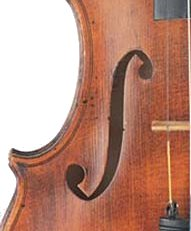
\includegraphics[width=4cm]{images/violin}
%
%
%\column{0.55\textwidth}
\begin{block}{}
\begin{center}
\begin{large}
 \insertsubtitle
\end{large}

\vspace{.1cm}

\begin{Large}
\textbf{\inserttitle}
\end{Large}


\vspace{.3cm}

{\insertdate}

\end{center}
\end{block}

\begin{center}
%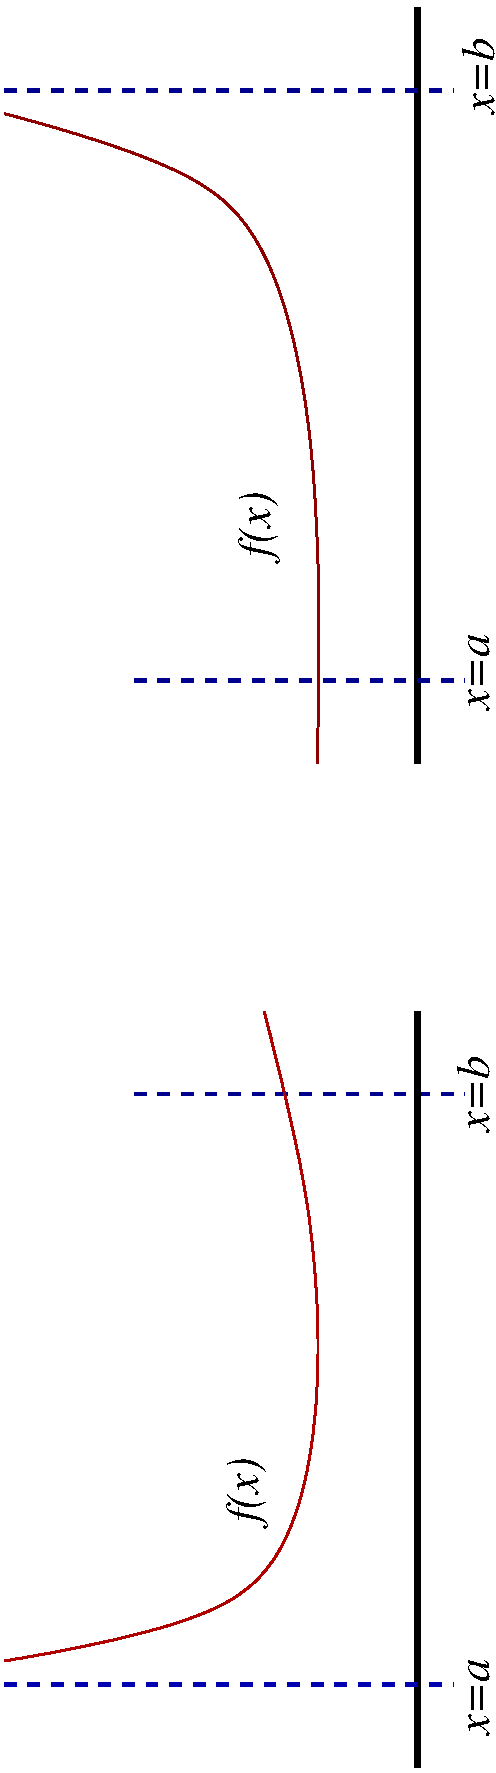
\includegraphics[width=3cm,angle=-90]{images/Improper2}
\end{center}


% \end{columns}

}

\frame{
  \frametitle{Topics of the day...}

%\begin{columns}[c]
%\column{0.5\textwidth}
 \tableofcontents
%\column{0.5\textwidth}


See also Sections 9.3 and 9.5 of Stewart.

%\end{columns}
}



\section{Recall: 1st Order Differential Equations}
\frame{

At the beginning of the course, we looked briefly at 1st Order Differential
Equations.

Later we  studied some  2nd order problems with constant
coefficients.

Now we return to 1st Order problems with non-constant coefficients.
These can't be solved with the simple substitution \eq{y=e^{rx}}:
we'll need to use the Techniques of Integration that we learnt over
that last 2 weeks.

}

\frame{

\begin{block}{}
As \Emph{1st Order Differential Equation} is of the form
\begin{center}
\eqd{\frac{dy}{dx} = f(x,y)}.
\end{center}
That is: the right hand side is some function of both \eq{x} and \eq{y}.

\pause
\Emph{Solving} the equation means expressing the relationship between
\eq{x} and \eq{y} in a manner not involving derivatives. 
\end{block}
\pause
The approaches that we will study are
\begin{enumerate}[<+->]
\item Separable DEs (today)
\item Homogeneous DEs 
\item Integrating Factors.
\end{enumerate}
}


%\section{Separable and Homogeneous 1st Order Equations}
\section{Separable  Equations}
\frame{


\begin{block}{}
A first order equation \eqd{\frac{dy}{dx} = f(x, y)} is \Bf{separable}
if we can write \eq{f(x)} as the product of some functions $g(x)$ and
$h(y)$. That is, it has the form 
\[
\frac{dy}{dx} =g(x)h(y).
\]
\pause
Such an equation can be solved by writing 
\[
\frac{1}{h(y)}dy = g(x)\,dx
\]
and integrating both sides:
\[
\int \frac{1}{h(y)}dy = \int g(x)\,dx
\]
\end{block}
}



\frame{
\begin{example}
Solve the equation \eqd{{\frac{dy}{dx}}=e^{x-y}}.
\end{example}

\vspace{4cm}
%\noindent\und{Solution}: We have $\disfrac{dy}{dx}=\disfrac{e^x}{e^y}$.
%Thus $e^y\,dy = e^x dx$, and 
%$$
%\int e^y\,dy = \int e^x\,dx \Longrightarrow e^y =- e^x + C.
%$$
%Thus solutions are given by $y(x)=\ln (e^x+C)$, for a constant $C$.

}

\frame{
\begin{example}
Solve the differential equation \eqd{\disfrac{dy}{dx}= \frac{6x^2}{2y + cos(y)}}.
\end{example}

\vspace{4.5cm}

}


\frame{
\begin{example}
Solve \eqd{\disfrac{dy}{dx}=\sqrt{y}\cos^2\big(\sqrt{y}\big)}.
\end{example}

\vspace{4.5cm}

%\noindent\und{Solution}: We have $\disfrac{1}{\sqrt{y}\cos^2\sqrt{y}}\,dy =
%dx$. Thus 
%$$
%\int\frac{1}{\sqrt{y}\cos^2\sqrt{y}}\,dy = \int\,dx.
%$$
%Let $u=\sqrt{y}$. Then $\disfrac{du}{dy}=\disfrac{1}{2}y^{-1/2}$ and
%$\disfrac{1}{\sqrt{y}}\,dy = 2\,du$. Thus 
%$$
%2\int \sec^2 u\,du = \int\,dx \Longrightarrow 2\tan u = x+C.
%$$
%Solution : $2\tan(\sqrt{y}) = x+C$.
}




\frame{
\begin{example}
Solve the equation $\disfrac{dy}{dx} = \frac{xy-2y+x-2}{x+3}$. 
\end{example}
\pause
\Bf{Solution}: This equation is separable : 
\[
\frac{dy}{dx} = \frac{(x-2)(y+1)}{x+3}\Longrightarrow
\frac{dy}{y+1}=\frac{x-2}{x+3}\,dx.
\]
Then...
\vspace{3.4cm}
%$$
%\int\frac{dy}{y+1} = \int\frac{x-2}{x+3}\,dx =
%\int\frac{x}{x+3}\,dx-2\int\frac{1}{x+3}\,dx. 
%$$
%If $u=x+3$ then $x=u-3$, $dx=du$ and 
%$$
%\int\frac{x}{x+3} = \int 1-\frac{3}{u}\,du = u - 3\ln |u| (+c).
%$$
%Now integrating gives 
%$$
%\ln |y+1| = x+3-3\ln |x+3|-2\ln |x+3| +C = x+3-5\ln |x+3| +C.
%$$

}

\frame{
\begin{example}%[MA211, Semester 1 2006, Q3 (d)]
Solve the differential equation
\[
\frac{dy}{dx} = -(y^2 + 2y +2)(x+1)\ln(x) \text{ with }
y(1)=-1
\]
\end{example}
\vspace{4cm}

}


\frame{

\begin{exercise}[21.1]
Find the general solution to the 1st order separable DEs
\begin{enumerate}[(i)]
\item \eqd{\frac{dy}{dx}= \frac{x}{y}} 
\hfill (ii) \eqd{\frac{dy}{dx}= \frac{y}{x}} 
\item[(iii)] \eqd{\dydx = y \ln(x)}
\hfill (iv)~ \eqd{ \frac{dy}{dx} = \frac{y}{2x}.}
\item[(v)] \eqd{ \frac{dy}{dx} = \frac{e^x}{\sin(y)}}
\hfill (vi)~ \eqd{  \frac{dy}{dx} = e^y{\sin(x)}.}
\item[(vii)] \eqd{\dydx = \frac{\ln(x)}{xy^2}}
\end{enumerate}
\end{exercise}
}

\frame{


\begin{exercise}[21.2]
Solve the following initial value problems:
\begin{enumerate}
\item \eqd{  \frac{dy}{dx} = 3 + e^y; \quad y(0)=1.}
\item \eqd{  \frac{dy}{dx} = \sinh(x)e^{-y} \quad y(0)=1};
\end{enumerate}
\end{exercise}

}



\section{Homogeneous Equations}
\frame{

Lectures 11 and 12 were concerned with solving \Emph{homogeneous}
2nd order differential equations with constant coefficient of the form:
\[
a y'' + b y' + cy = \alert{0}.
\]
Here the term   \Emph{homogeneous} means that the right-hand side of
the equation is \alert{0}.

For first-order problems, we have a different meaning of homogeneous:
if the right-hand side is a function of both \eq{x} and \eq{y}, but
can be written in terms of a single function \eq{v=y/x}.

}

\subsection{Homogeneous Functions}
\frame{
\begin{definition}
A function \eq{f(x,y)} is \Bf{homogeneous} \Emph{of degree \eq{k}} if
for every real number \eq{t} we have 
\[
f(tx, ty) = t^k f(x,y).
\]
\end{definition}

\pause

To work out if a function is homogeneous
\begin{enumerate}
\item Write down \eq{f(tx, ty)} 
\item Rearranged to get \eq{t^kf(x,y)} for some number \eq{k}
\item This tells you that the function is  homogeneous
  \Emph{and} its degree.
\end{enumerate}

\pause

\Bf{Important:} When the function is \emph{homogeneous of degree
  \eq{0}} we can make the substitution \eqd{v = \frac{y}{x}} and
rearrange to get   a function just in terms of \eq{v}.

}

\frame{

\begin{example}
For each of the following, determine if they are homogeneous. If they
are homogeneous, then to what degree?
\begin{enumerate}
\item \eqd{f = x^2 + xy + y^2} 

~

\item \eqd{f = \frac{xy + y^2}{x^2}}

~

\item \eqd{f = x^2 + y } 

~

\item \eqd{f = \frac{y}{xy}}.
\end{enumerate}
\end{example}
}

\frame{

\begin{exercise}[21.3]
For each of the following, determine if they are homogeneous and to
what degree.
\begin{enumerate}
\item \eqd{f = \sqrt{x^2 + y^2}} 
\item \eqd{f = \frac{x^2 + xy}{xy + y^2}}
\item \eqd{f = xy^2 } 
\item \eqd{f = \frac{2xy}{x^2 + y^2}}
\item \eqd{f = \frac{y}{x-y}}.
\end{enumerate}
\end{exercise}
}

\end{document}


\subsection{Solving homogeneous DEs}
\frame{

Given a first order differential equation \eqd{\frac{dy}{dx}=f(x,y)}
where \eq{f(x,y}) is  \Emph{homogeneous of degree \alert{0}},

\begin{enumerate}
\item Let \eqd{v = \disfrac{y}{x}} and find the function \eq{h} such
  that
\eqd{ h(v) = f(x,y).}

\item  Because  we have \eqd{y=vx}, differentiate to get:
\eqd{\frac{dy}{dx} = v + x \frac{dv}{dx}}

\item Substitute into the original differential equation:\\
\qquad \eqd{ v + x\disfrac{dv}{dx} = h(v).}

\item This equation involving \eq{v} and \eq{x} is separable:
\[ \frac{1}{h(v)-v}dv=\frac{1}{x}dx\]

\item Solve it in the same way we solve the separable problems from
  last week.
\end{enumerate}
}

\frame{

\begin{example}
Solve the equation $\disfrac{dy}{dx}=\disfrac{xy+y^2}{x^2}$.
\end{example}

%\und{Solution}: $f(tx,ty) = f(x,y)$ so \eq{f} is homogeneous of degree
%\alert{0}. \\
%3Write $v = \disfrac{y}{x}$. Then $\disfrac{dy}{dx} = v +
%x\disfrac{dv}{dx}$ and 
%$$
%v + x\disfrac{dv}{dx} = v+v^2\Longrightarrow x\disfrac{dv}{dx} = v^2.
%$$
%Thus 
%$$
%\frac{1}{v^2}\,dv = \frac{1}{x}\,dx\Longrightarrow
%\int\frac{1}{v^2}\,dv = \int\frac{1}{x}\,dx.
%$$
%Hence 
%$$
%-\frac{1}{v} = \ln |x|+C\Longrightarrow v = \frac{y}{x} =
%\frac{-1}{\ln |x|+C}.
%$$
%Solution : $y = \disfrac{-x}{\ln |x|+C}$. 

\vspace{3cm}

}

\frame{
\begin{example}
Solve the following initial value problem:
\[ 
  \frac{dy}{dx} = \disfrac{x^2 + xy}{xy + y^2}, \qquad y(2)=1.
\]
\end{example}
\vspace{4cm}
}

\frame{
\begin{example}[Autumn  exam 07/08, Q4(iii)]

Solve the following differential equation:
\[ 
  2xy \frac{dy}{dx} = x^2 + y^2, \qquad y(2)=2.
\]
\end{example}
\vspace{4cm}
}

\frame{
\begin{exercise}
Find the general solution to the following differential equations:
\begin{enumerate}
\item \eqd{  \frac{dy}{dx} = \disfrac{x + y}{x - y}.}
\item \eqd{  \frac{dy}{dx} = \disfrac{xy}{x^2 +2y^2}.}
\end{enumerate}
\end{exercise}

\begin{exercise}
Solve the following initial value problems:
\begin{enumerate}
\item \eqd{  \frac{dy}{dx} = \disfrac{x^2 + xy + y^2}{x^2}; \quad y(1)=1.}
\item \eqd{  \frac{dy}{dx} = \disfrac{x^3 + 3xy^2}{3x^2y + y^3};
    \qquad y(1)=-1}
\end{enumerate}
\end{exercise}

}

\end{document}
